\subsection{Description}
This mono effect mimics purposefully distorts a signal to create nonlinear effects. Two types of distortion exist - soft clipping and hard clipping. Soft clipping mimics an older era of vacuum tubes, whereas hard clipping mimics the harsher sound of a transistor amplifier.

\subsection{Applications}
Distortion is common technique used in modern or rock music to create a harsher, richer sound.

\subsection{Principles of Operation}
Distortion is simply applying a nonlinear gain to a signal so that the input-output transfer curve is altered. Soft clipping has a smoother, continuous transfer curve, while hard clipping is discontinuous. Figure \ref{fig:distortion-transfer-curves} shows the transfer curves for soft and hard clipping.
\begin{figure}[ht]
    \centering
    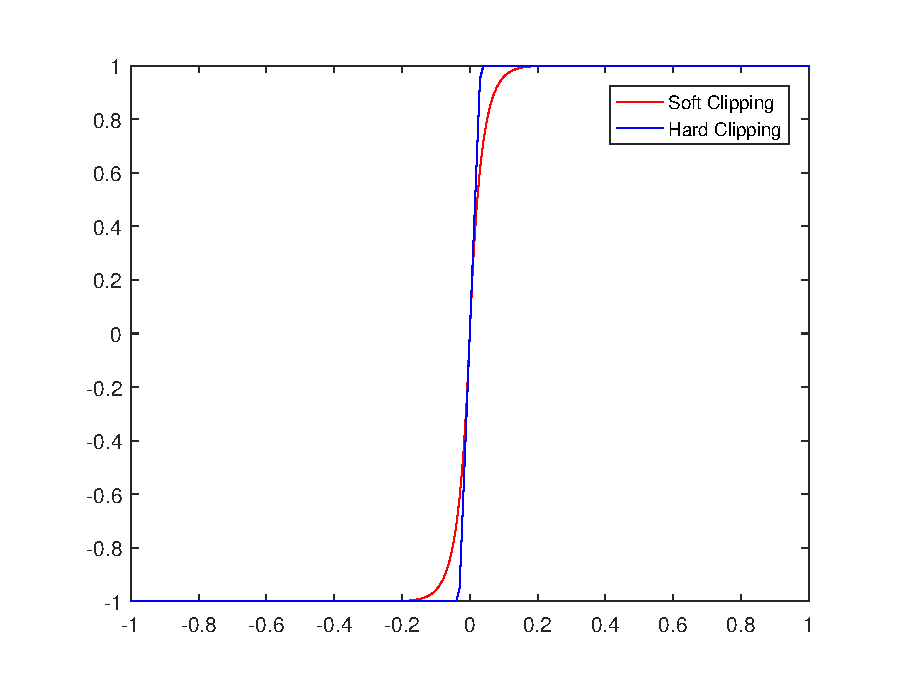
\includegraphics[scale=0.6]{distortion-transfer-curves.eps}
    \caption{Input-Output Transfer Curves for Soft and Hard Clipping}
    \label{fig:distortion-transfer-curves}
\end{figure}
Soft clipping can be implemented using Equation \ref{eq:soft-clipping}, and hard clipping uses Equation \ref{eq:hard-clipping}.
\begin{equation}
    y = \mathrm{sgn}(x) (1 - e^{-|Gx|})
    \label{eq:soft-clipping}
\end{equation}
\begin{equation}
    y =
    \begin{cases}
        -1 & \quad Gx \leq -1 \\
        Gx & \quad -1 < Gx < 1 \\
        1 & \quad Gx \geq 1 \\
    \end{cases}
    \label{eq:hard-clipping}
\end{equation}

\subsection{Implementation}
Distortion was implemented in MATLAB (see \href{run:../clipping.m}{clipping.m}) using the equations in the previous section. The gain is specified in dB, and the script reinterprets this parameter as the linear gain, $G$.

\subsection{Demo and Discussion}
The effect is best heard on the ``Hero'' \href{run:../InputAudio/22-001 Original Vocal.wav}{vocal track}. Soft clipping was applied for \href{run:../OutputAudio/clipping_22-001 Original Vocal_{pre-gain=10}{soft-clipping=1}.wav}{10 dB}, \href{run:../OutputAudio/clipping_22-001 Original Vocal_{pre-gain=30}{soft-clipping=1}.wav}{30 dB}, \href{run:../OutputAudio/clipping_22-001 Original Vocal_{pre-gain=50}{soft-clipping=1}.wav}{50 dB}. The output sounds particularly harsh at 50 dB. However, it is possible to distinguish between an extremely loud soft clipping signal and the harshness of hard clipping, even at only \href{run:../OutputAudio/clipping_22-001 Original Vocal_{pre-gain=30}{soft-clipping=0}.wav}{30 dB}. Figures \ref{fig:soft-clipping-output} and \ref{fig:hard-clipping-output} show the output of vocal sample for both distortion styles at 30 dB.
\begin{figure}[ht]
    \centering
    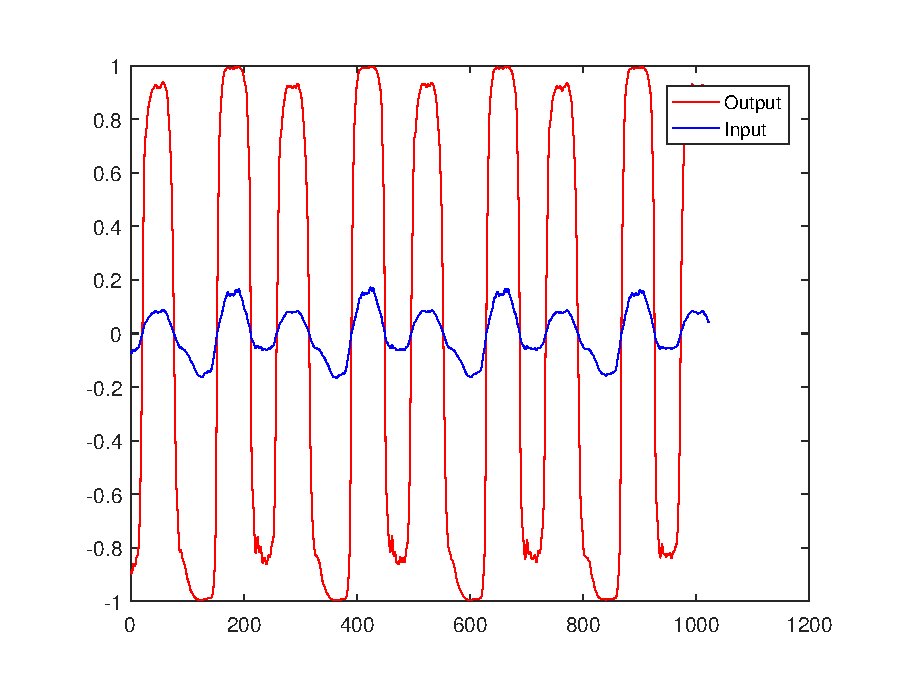
\includegraphics[scale=0.6]{soft-clipping-waveform.eps}
    \caption{Output at 30 dB with Soft Clipping}
    \label{fig:soft-clipping-output}
\end{figure}
\begin{figure}[ht]
    \centering
    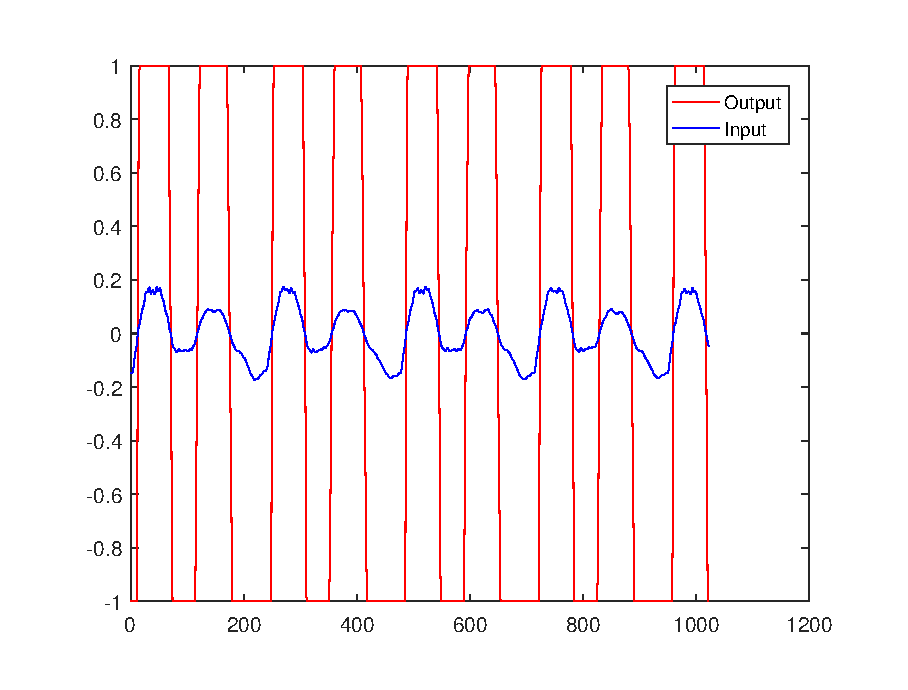
\includegraphics[scale=0.6]{hard-clipping-waveform.eps}
    \caption{Output at 30 dB with Hard Clipping}
    \label{fig:hard-clipping-output}
\end{figure}

\subsection{Further Exploration}
Though distortion can be found in almost any rock song, a great song to contrast a distorted guitar versus a clean guitar is Led Zeppelin's \href{https://www.youtube.com/watch?v=0Az-TuYb4h0}{Over the Hills and Far Away}. Around 1:40, you can hear some cleaner guitar, but very soon, Jimmy Page transitions to the harder riff of the song, and the distortion kicks in.